%!TEX root = thesis.tex
\chapter{Introduction}\label{c:1}
At high temperature, an isolated collection of molecules at a low enough volume fraction is a fluid and thus is a uniform system; the probability of finding any molecule at any specific position is a constant and only depends on the density of the particles.
As this system is invariant under all possible rotations and translations, we say that the system has complete continuous translational and rotational symmetry.
If we lower the temperature, the system will eventually develop order, where the individual molecules have a preferred local arrangement.
For this example, lowering the temperature will eventually force the system to transition from a fluid phase to a crystalline phase, where the molecule positions make up a periodic lattice.
Thus, the system is now only invariant with respect to a discrete set of translations and rotations.
Here, the system breaks the continuous symmetry of the isotropic phase in order to achieve the crystalline phase.
Hence, the ordered phase has lower symmetry than the isotropic phase.

The advent of order as a result of continuous symmetry breaking is general and is a hallmark of transitions between a multitude of different phases.
In addition, the phases do not have to be formed by collections of molecules; they can be built from a variety of constituent units, from angstrom-scale atoms, to micron-scale colloids, or even larger building blocks.
Regardless of the constituent particles, the isotropic-to-crystalline phase transition in three-dimensions (3D) breaks continuous translational and rotational symmetry in all directions.
However, a system can also transition from an isotropic phase to a phase where the continuous translational and rotational symmetry in not broken in all directions.
For example, an isotropic-to-smectic phase transition in 3D breaks continuous translation symmetry in only one direction and continuous rotational symmetry in two directions, while the isotropic-to-uniaxial nematic and isotropic-to-ferromagnetic transitions break no translational symmetries and only break rotational symmetry in two directions~\cite{RN175}.
Breaking continuous translational symmetry results in positional order while breaking continuous rotational symmetry results in orientational order.

With the development of order comes the rigidity needed to maintain that order.
For example, crystalline and smectic materials do not flow easily due to their broken translational symmetries.
However, nematics with their continuous translational symmetries flow far easier; the constituent particles only need to maintain their orientation and not their position.
In addition, systems with anisotropic order must have a correspondingly anisotropic rigidity.
Consider a smectic phase with its broken translational symmetry in one direction, given by the unit vector $\bm{\sigma}$\fxnote{Schematic to define nematic and smectic stuff.}.
Along $\bm{\sigma}$, the material will resist flow like a crystal, but will flow easily like a fluid in the plane orthogonal to $\bm{\sigma}$.
Similarly, even though a uniaxial nematic has continuous translation symmetry in all directions, it still has rigidity as the nematic must maintain its two-fold orientational order.
This rigidity is thus anisotropic, reflecting the nematic's anisotropic rotational symmetry.
This phenomenon is not limited to the rigidity; in general, the properties of a phase will reflect its symmetries.
For example, ordered materials often exhibit birefringence, where the index of refraction is anisotropic.
A light wave incident on a birefringent material will thus encounter an index of refraction that depends on the direction and polarization of the light wave~\cite{RN175}.

Ordered materials can also have defects, defined generally as locations in the material where the preferred local arrangement is not satisfied.
Belying their name, defects are not necessarily undesirable; in fact, they can have important consequences for the physics of the phase, which could be exploited to achieve specific properties.
For example, joining two crystalline domains of incompatible orientations results in defects forming a border, or grain boundary, between the two domains.
In a crystalline material, these grain boundaries affect the moduli of the material, and are even responsible for the phenomenon of ``work hardening,'' where plastically deforming the material increases the magnitude of the shear modulus.
This is commonly done to create durable objects and sculptures from copper and other ductile metals.
The plastic deformations cause isolated defects and grain boundaries to proliferate within the material; however, as the defect density rises, so does the energy required to generate each new defect, resulting in an increased resistance to deformation that further reflects in the increase of the shear modulus.

In addition, defects can also directly mediate phase transitions, as in the celebrated Kosterlitz-Thouless-Halperin-Nelson-Young (KTHNY) theory of melting in 2D~\cite{RN161,RN162,RN163}.
Here, the increase in symmetry when a 2D crystalline phase melts to the isotropic phase is a two-step process.
First, pairs of rotational defects, or disclinations~\cite{RN61,RN203}, proliferate, driving the crystalline phase into an intermediate hexatic phase characterized by six-fold orientational order.
Second, these disclination pairs unbind, transforming the hexatic phase into the isotropic phase.
Furthermore, defects in soft matter have been used as tools to investigate a wide range of phenomena from knot theory~\cite{RN156,RN277} to controlled self-assembly~\cite{RN43,RN50,RN150,RN157}, to hierarchical materials~\cite{RN164,RN159,RN27}.

Apart from their effect on physical systems or their use as tools, defects are fascinating objects in their own right as they are extremely sensitive to the intrinsic geometry of the space they inhabit.
Consider, for example, densely packing rods on a plane.
In order to maximize the entropy of the system, the rods need to align along the same direction, breaking continuous rotational symmetry and yielding the the two-fold order of the uniaxial nematic phase~\cite{RN204}.
We can characterize this preferred local alignment with a director, $\mathbf{n}$, where $\mathbf{n} = \mathbf{-n}$, reflecting the inversion symmetry of the 2-fold order.
Clearly, it is easy to fill space on the plane with a homogeneous director field, as shown schematically in Figure~\ref{f:1-RodsPlane}(A).
However, if we now try to pack rods on the surface of a sphere, for example along either the latitude or longitude lines of the Earth's globe [Figure~\ref{f:1-RodsPlane}(B)], we see that there are defects in the order that correspond to the singular points at the poles, where $\mathbf{n}$ is undefined.
Since you ``cannot comb a hairy ball,'' the presence of singularities is no accident --- it is a consequence of confining the nematic to the surface with the topology of a sphere~\cite{RN209,RN169}.
\begin{figure}
  \centering
  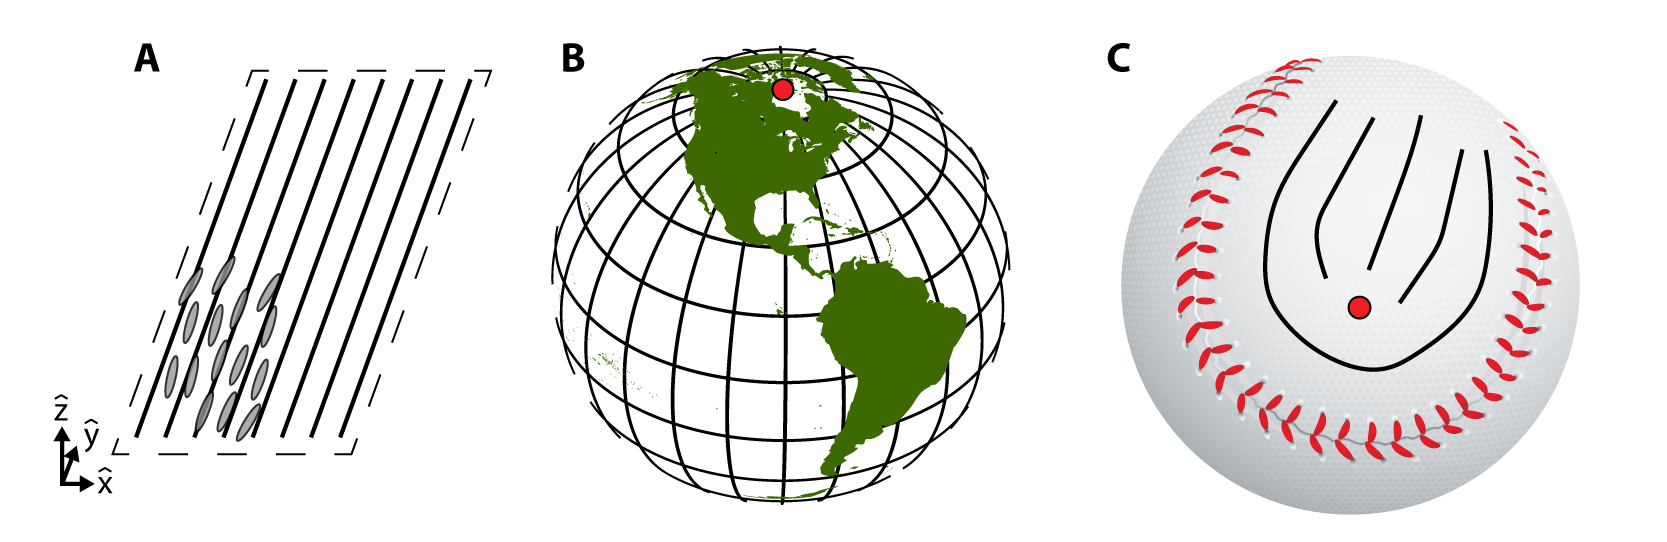
\includegraphics{figures/C1/Ch1-Figs_RodsPlane.png}
  \caption{Packing rods in two dimensions.
  (A-C), Rod-like particles preferentially align along a commmon axis, given by the black lines.
  (A) On a plane, the alignment can be homogeneous everywhere.
  (B,C) On a sphere, there must be singularities (${\color{red} \bullet}$) in the alignment directions, as shown for alighment directions along (B) the latitude or longitude lines on a globe and an alignment direction along (C) the stitching on a baseball.
  Note that there while only one singularity is visible in (B,C), there are 2 singularities in (B) and 4 in (C).}\label{f:1-RodsPlane}
\end{figure}\fxnote{Discontinuous lines on the plane.}

To formally relate the topology of the sphere with the presence of singularities, we need a few topological notions.
The sphere is an example of a differentiable surface that is compact, has no boundary, and is orientable.
Compact surfaces must both be bounded and contain their limit points.
Here, the term ``bounded'' means the surface has some finite size and is distinct from whether or not the surface has a boundary.
The boundary of a surface is defined as the set of points that can be approached from both the interior and the exterior of the surface.
Finally, orientable surfaces have a defined normal vector everywhere.
For example, 2D Euclidean space, denoted as $\mathbb{R}^2$, is a surface but it is not bounded and thus it is not compact.
With $\mathbf{r}$ a vector in $\mathbb{R}^2$, the 2D open unit disc $|\mathbf{r}| < d$ is not compact since it does not contain the circle with radius $d$.
However, the 2D unit disc $|\mathbf{r}| \leq d$ satisfies both conditions and thus is compact.
In addition, we see that $|\mathbf{r}| \leq d$ has a boundary $\partial \mathbf{r}$ at $|\mathbf{r}| = d$, as $\partial \mathbf{r}$ can be approached by points both the interior and exterior of the disc.
We call compact surfaces without a boundary closed surfaces.
Finally, all of these examples are also orientable; it is trivial to define the surface normal everywhere.
\begin{figure}
  \centering
  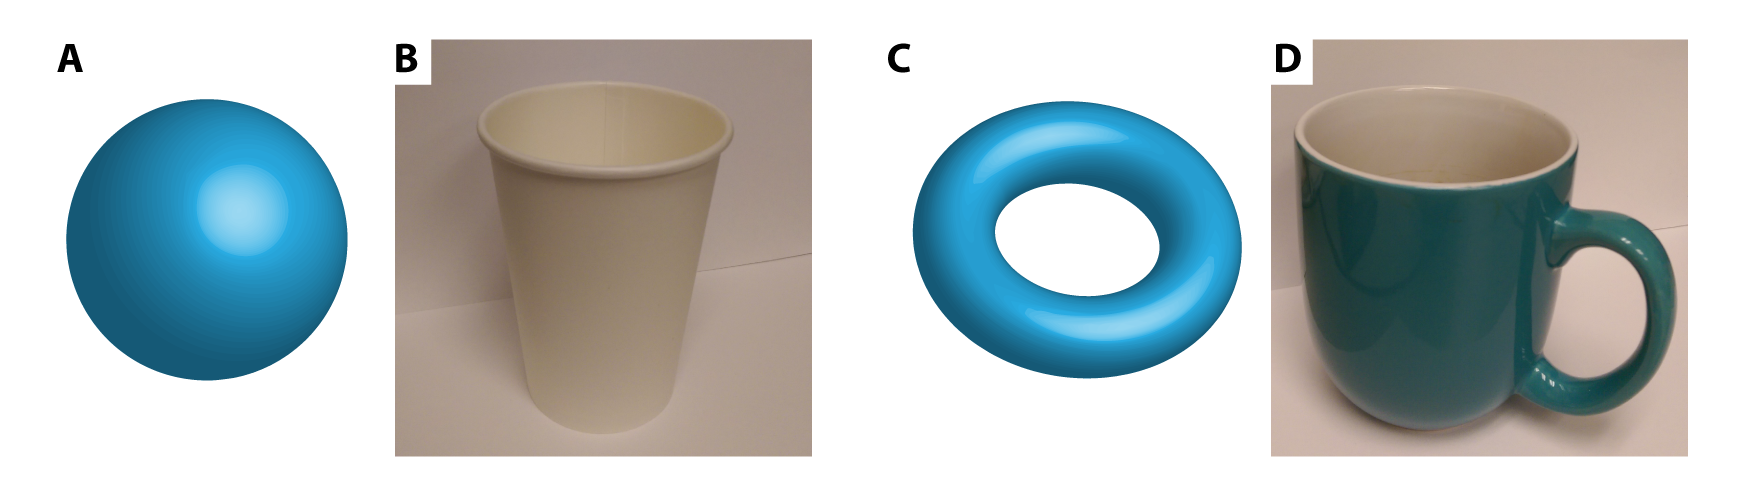
\includegraphics{figures/C1/Ch1-Figs_ChiObjects.png}
  \caption{Closed surfaces with the same Euler characteristic are homeomorphic. (A,B) Closed surfaces with no handle like a (A) sphere and a (B) cup can be continuously deformed into each other.
  (C,D) Closed surfaces with a single handle like a (C) torus and a (D) coffee mug can be continuously deformed into each other.
  However, the surfaces in (A,B) cannot be continuously deformed in the surfaces in (C,D) as the process of adding a handle breaks the surface.}\label{f:1-ChiObjects}
\end{figure}

We can characterize the topological properties of a surface with its Euler characteristic, $\chi$, which we can calculate using the Gauss-Bonnet theorem.
For a closed surface the theorem states that~\cite{RN23}:
\begin{equation}
  \chi = 2(1-g),\label{e:1-GB1}
\end{equation}
where $g$ is the genus, or number of handles, of the surface.
The Euler characteristic is a topological invariant --- continuously deforming a surface, i.e.\ under a homeomorphism, does not change its Euler characteristic.
A homeomorphism is continuous function with a continuous inverse that maps one topological space to another.
For example, a sphere has no handles, thus $g = 0$ and $\chi=2$.
Since a homeomorphism preserves the topological properties, any surface with $g=0$ is topologically equivalent, or homeomorphic, to the sphere, and therefore also has $\chi=2$.
For example, as pictured in Figure~\ref{f:1-ChiObjects}(A,B), a sphere is homeomorphic to a cup, as neither have handles.
Similarly, the torus and the coffee mug pictured in Figure~\ref{f:1-ChiObjects}(C,D), respectively, are also homeomorphic to each other.
However, the sphere [Figure~\ref{f:1-ChiObjects}(A)] and the torus [Figure~\ref{f:1-ChiObjects}(C)] are not homeomorphic as we cannot add a handle to the sphere without breaking its surface.

Thus, we can extend the statement, ``you cannot comb a hairy ball'' to, ``you cannot comb a hairy surface with $\chi=2$.''
In fact, any attempt to do so will necessarily result in the presence of singularities.
In an orientation field like a director field, singularities are called ``disclinations''.
We can characterize a disclination by how much the director rotates along a closed contour encircling the disclination.
For a contour $\partial A$ and the angle $\phi(\mathbf{r})$ parameterizing the director field, with $\mathbf{r}$ the position vectors of a point on the surface, we can calculate~\cite{RN23,RN153,RN203}:
\begin{equation}
  s = \frac{1}{2 \pi}\oint_{\partial A} \textrm{d}\mathbf{r} \cdot \nabla\phi(\mathbf{r}) = \frac{1}{2\pi} \oint_{\partial A} \textrm{d} \phi.\label{eq:1-topCharge}
\end{equation}
If we map $\phi$ on $\partial A$ onto points on $\mathbb{S}^1$, the unit circle, we see that $s$ is the number of times the director field wraps the unit circle.
Since we cannot eliminate the enclosed disclination with continuous deformations of the director, disclinations are topological and $s$ is known as the winding number, or ``topological charge.''
Regardless of aligning rods along the latitudes or the longitudes on the Earth's globe, the director along a contour encircling either pole rotates by $2 \pi$, as depicted in Figure~\ref{f:1-TopCharge}(A).
Thus, both the north and the south poles have charge $s = +1$, bringing the total charge on the surface to $+2$.
The formal statement connecting a vector or director field on a closed surface with the topology of the surface is the Poincar\'e-Hopf theorem~\cite{RN23}:
\begin{equation}
  \sum\limits_{i = 1}^{N} s_i = \chi,\label{e:1-PH}
\end{equation}
where $N$ is the number of disclinations, each of topological charge $s_i$.

Thus, $s \in n/2$, where $n \in \mathbb{Z}$, the integers, for nematic order, while $s = n$ for polar order.
For example, the defect structure in Figure~\ref{f:1-TopCharge}(B) has $s = +1/2$ and can exist in a nematic director field, where $\mathbf{n} = \mathbf{-n}$.
Attempting to construct such a disclination with a vector field, as illustrated by following the vectors as they go from blue to cyan along the red contour in Figure~\ref{f:1-TopCharge}(C), we see that we get a $\pi$-flip and the vector field is not continuous.
Not also that the Poincar\'e-Hopf Theorem only requires the total charge on the surface to be equal to $\chi$; we can construct a director or a vector field on a closed surface with any combination of defects so long as the total topological charge is equal to $\chi$.

Physical ordered systems constrained to a closed surface must then minimize their free energy while complying with the constraint imposed by the Poincar\'e-Hopf theorem.
\begin{figure}
  \centering
  
\includegraphics{figures/C1/Ch1-Figs_TopCharge.png}
  \caption{Topological charge of disclinations.
  (A), The director rotates by $2\pi$ along the contour enclosing the singularity (${\color{red} \bullet}$), giving $s = +1$ for both disclinations.
  (B) The director rotates by $\pi$ along the contour enclosing the singularity (${\color{red} \bullet}$), giving $s = +1/2$.
  (C) Attempting to construct an $s = +1/2$ disclination for a vector field results in a discontinuity in the vector field along the contour.
  This is seen by following the red contour as the vectors go from blue to cyan.}\label{f:1-TopCharge}
\end{figure}

For an orientationally ordered phase where the particles prefer to align parallel to each other, we can write the free energy in terms of the cost of distorting the material from the homogeneously-aligned state.
In the continuum limit, this distortion free energy is a functional of the orientation field,
\begin{equation}
  F_d = \frac{1}{2} k_F \int \textrm{d}^2\mathbf{r} \, |\nabla \phi(\mathbf{r})|^2,\label{e:2-XY}
\end{equation}
where $k_F$ is the elastic constant governing the cost of distortion.
If we have polar order described by a vector field, then Eq.~\ref{e:2-XY} is the classical 2D X-Y model governing spins on a fixed lattice~\cite{RN175}; for nematic order, Eq.~\ref{e:2-XY} is the 2D Frank-Oseen free energy~\cite{RN61} in the 1-constant approximation~\cite{RN33}.

Nematics on a sphere were predicted~\cite{RN42,RN104,RN43} to minimize the free energy not with two $s=+1$ defects [Figure~\ref{f:1-RodsPlane}(B)] but with four $s=+1/2$ defects arranged on the vertices of a tetrahedron [Figure~\ref{f:1-RodsPlane}(C)].
Prior work in our group addressed this situation experimentally using glass-based microfluidic devices to fabricate double emulsions~\cite{RN272}, with a shell of nematic liquid crystal (NLC) between an inner water droplet and an outer water continuous phase~\cite{RN105,RN45}.
By decreasing the osmotic pressure in the outer continuous phase of the nematic shells, swelling of the inner droplet was induced, decreasing the thickness of the NLC shell to create an experimental realization of a 2D nematic on the surface of a sphere~\cite{RN45}.
In this thin shell limit, the four $s = +1/2$ defects arranged on the vertices of a tetrahedron was observed; see Figure~\ref{f:1-Shells}(A,B).
\begin{figure}
  \centering
  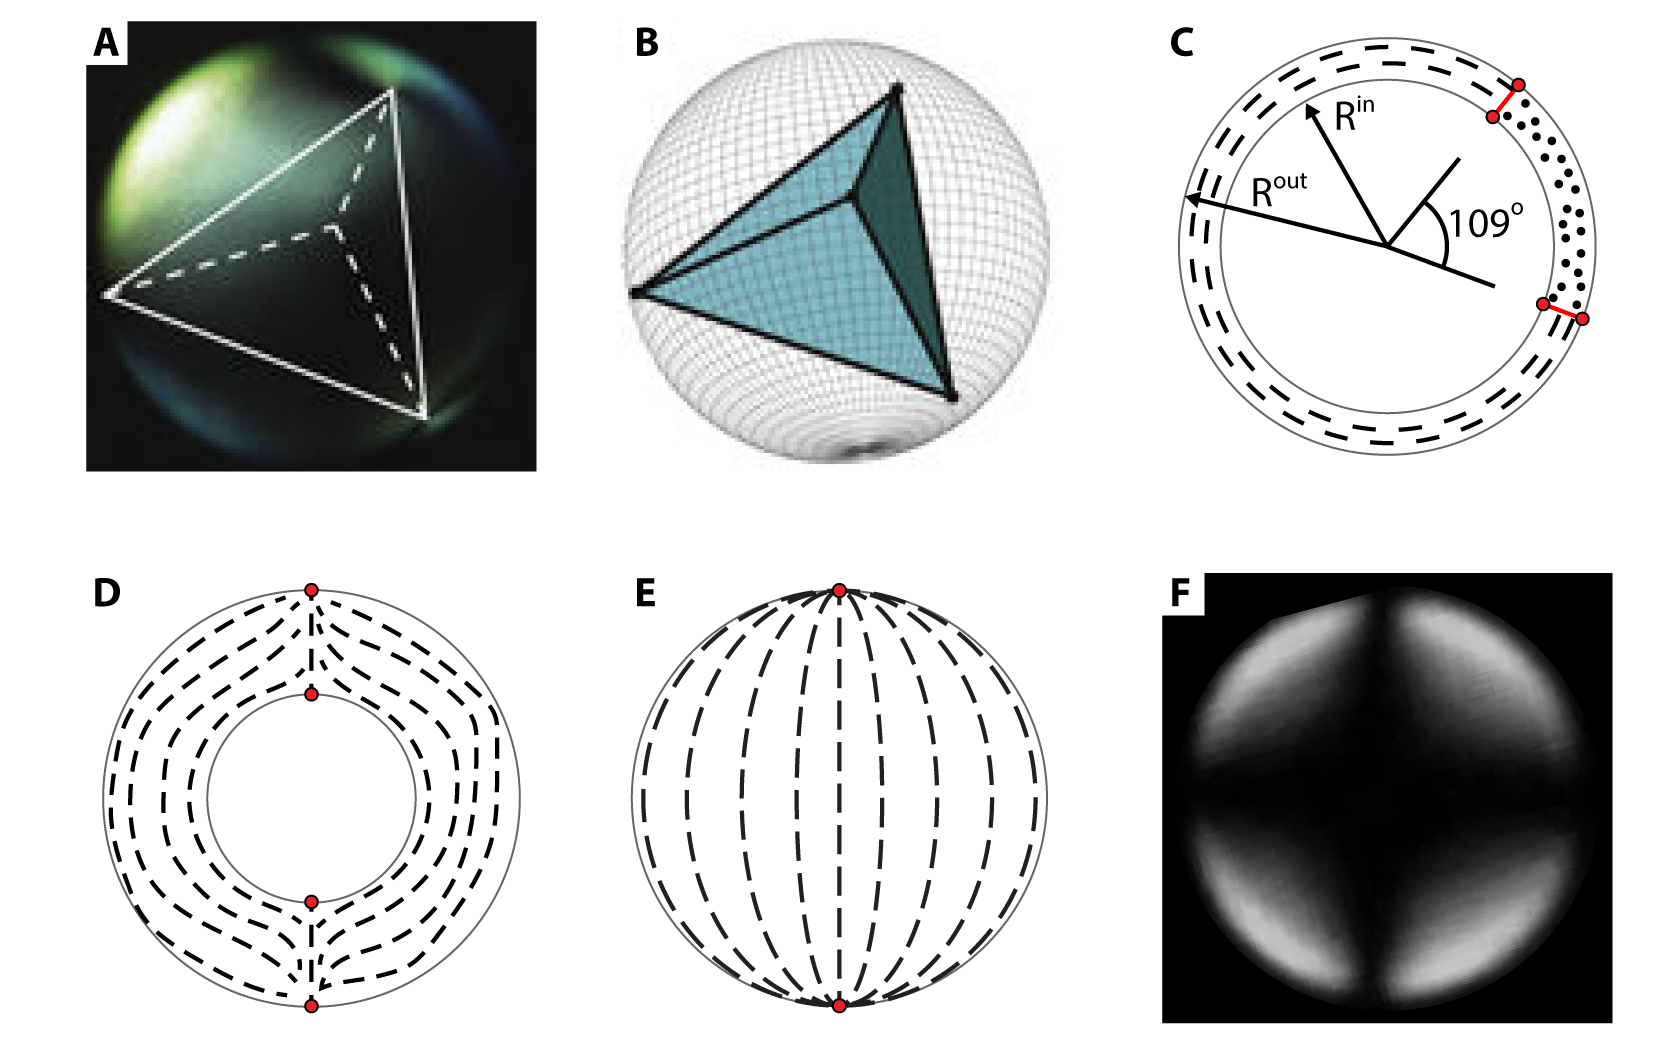
\includegraphics{figures/C1/Ch1-Figs_Shells.png}
  \caption{Shells of nematic liquid crystal.
  (A-C) Thin shells of NLC have four $s = +1/2$ defects, with an experimental crossed-polar image in (A), the tetrahedron highlighted in (B), and a cross-section schematically showing the director configuration in (C).
  The cross-section is of a great circle containing two $s = +1/2$ defects (${\color{red} \bullet}$) on both the inner and outer surface of the shell, with a red singular line connecting corresponding disclinations.
  The disclinations occupy the vertices of a tetrahedron and thus are separated by $109^{\circ}$ in the cross-section.
  (D) Cross-section of the director configuration in a thick shell. Here, the two $s = +1$ disclinations (${\color{red} \bullet}$) on each surface are no longer connected by a singular line.
  (E,F) As $R^{in}\rightarrow 0$, the thick shell becomes a bipolar droplet, with a cross-section of the director field in (E) and a corresponding crossed-polar image in (F).}\label{f:1-Shells}
\end{figure}

However, this arrangement of $s = +1/2$ defects only exists in thin enough shells, as characterized by the relative shell thickness $h' = (R^{out}-R^{in})/R^{out}$, with $R^{in}$ and $R^{out}$ the inner and outer radius of the nematic shell, as defined schematically in Figure~\ref{f:1-Shells}(C).
As $h'$ increases, the shell also becomes inhomogeneous due to density differences between the inner droplet and the NLC shell.
This thickness heterogeneity drives defects to the thinnest portion of the shell; this means that the $s = +1/2$ are no longer in a tetrahedron.
In addition, as $h'$ increases, the shell can no longer be considered 2D.

The situation is now 3D and there are two spherical interfaces where the topological charge on the interface is constrained by the Poincar\'e-Hopf theorem with a bulk region between the two surfaces filled with NLC.
Each $s = +1/2$ defects on the outer surface is connected to their corresponding $s = +1/2$ disclination on the inner surface via a singular line that propagates through the bulk, as depicted schematically in Figure~\ref{f:1-Shells}(C) for a great circle containing two $s = +1/2$ disclinations on each surface.
As $h'$ increases, so does the cost of each singular line.
Eventually, as $h'\gtrsim 1/2$, the cost of propagating the singular lines through the bulk is too great and the pairs of $s = +1/2$ disclinations on each surface transition to one $s = +1$ disclination~\cite{RN105}, known as a boojum~\cite{RN273}.

Unlike the $s = +1/2$ defects, the boojums are not connected by a singular line; instead, the director in the shell region ``escapes in the third dimension'' and acquires a component along the radius of the droplet, removing all the singularities in the bulk.
The increased energetic cost of a single boojum as compared to two $s = +1/2$ defect is compensated by the energetic decrease of removing the singular regions in the bulk of the shell.
This is depicted schematically for a two boojums on each surface for the special case of a homogeneous shell in Figure~\ref{f:1-Shells}(D).
For a heterogeneous thickness, the boojums will migrate towards the thinnest portion of the shell.
In addition, the shells are not restricted to either 4 $s = +1/2$ disclinations of two $s = +1$ boojums; our group also observed hybrid shells with two $s = +1/2$ disclinations and a single boojum.
For $h' = 1$, there is no inner water droplet and we have a single droplet of NLC in a continuous water phase, with the boojums on opposite poles.
This director arrangement is the classic bipolar configuration, with the director field and associated crossed polar image shown in Figure~\ref{f:1-Shells}(E,F), respectively.

Note that even if Eq.~\ref{e:2-XY} favors a homogeneous orientation field, corresponding to the zero energy configuration, sometimes distortions are unavoidable due to the topological constraints imposed by the surface.
However, ordered materials are also sensitive to the local geometry.\fxnote{HERE}
For example, consider once more rods packed on a plane with a homogeneous director field, as shown schematically in Figure~\ref{f:1-ParallelTransport}(A).
If we change the geometry and introduce a hemispherical ``bump'' in the plane, as illustrated in Figure~\ref{f:1-ParallelTransport}(B), evenly-spaced director lines on the plane do not maintain their spacing on the bump.
Thus, we no longer have a homogeneous director everywhere on the surface.
This inability to maintain the preferred local order due to the geometry of the surface is called ``geometrical frustration''.\fxnote{modify and introduce the antiferromagnetic tirangular alttice with a schematic}
\begin{figure}
  \centering
  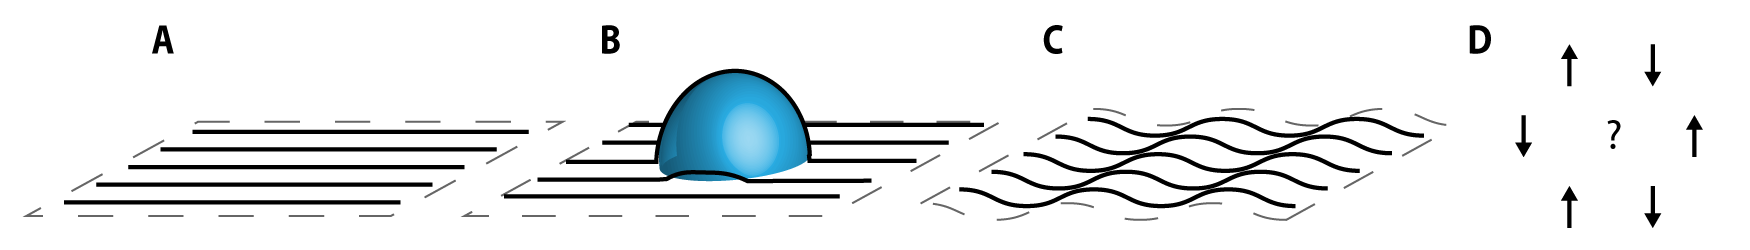
\includegraphics{figures/C1/Ch1-Figs_ParallelTransport.png}
  \caption{Geometrical frustration comes from Gaussian curvature.
  (A), A flat plane can support a homogeneous director field, indicated by the black lines.
  (B), Adding a hemisphere to the plane disrupts the homogeneous state, the Gaussian curvature of the hemisphere makes a distortion-free state impossible.
  (C), Modulating the surface with a sine wave adds mean curvature but not Gaussian curvature to the surface; the homogeneous state on the surface is still possible.}\label{f:1-ParallelTransport}
\end{figure}\fxnote{discontinuous lines}

An important aspect of the local geometry of a surface is its curvature; consider a curve constrained to lie in $\mathbb{R}^2$, $\mathbf{r}(s)$, with $s$ the arclength parameter.
Such an example of a planar curve is drawn schematically in Figure~\ref{f:1-Curvature}(A).
The unit tangent to the curve at $s$ is given by $\mathbf{T}(s) = \textrm{d} \mathbf{r}(s)/\textrm{d}s = \mathbf{r}'(s)$, and the local curvature $\kappa(s)$ by $\mathbf{k}(s)\kappa(s) = \mathbf{T}'(s) = \mathbf{r}''(s) $, with $\mathbf{k}(s)$ the unit normal vector to the curve [see Figure~\ref{f:1-Curvature}(A)].\fxnote{prove it?}
$\kappa(s) = 1/R(s)$, where $R(s)$ is the radius of the osculating circle, or circle that best approximates $\mathbf{r}(s)$ at $s$.
This radius is commonly known as the ``radius of curvature'' at $s$.
The sign of the curvature relates to the direction $\mathbf{k}$ rotates as $s$ increases: if $\mathbf{k}$ rotates counterclockwise, then $\kappa > 0$, while if $\mathbf{k}$ rotates clockwise, $\kappa < 0$.
The osculating circles and associated radii of curvature are drawn in blue and red in Figure~\ref{f:1-Curvature}(A) for a point with negative curvature and a point with positive curvature.

Now consider a 2D orientable surface given by $\mathbf{R}(u^1,u^2) \in \mathbb{R}^3$, with $(u^1,u^2) \in U \subset \mathbb{R}^2$ local coordinates on the surface, with $U$ a local coordinate patch.
We define a normal section at a point $\mathbf{r} \in U$ on the surface as the planar curve resulting from the intersection between the surface and a plane containing.
Since the orientation of the plane is not unique, there are infinitely many planes that can contain $\mathbf{k}(\mathbf{r})$, and therefore infinitely many normal sections at a given point $\mathbf{r}$.
The curvature of a given normal section at $\mathbf{r}$ is called the normal curvature.
A normal section, the plane containing $\mathbf{k}$, and the osculating circle whose $R$ determines the normal curvature $\kappa(s)$ are drawn schematically for an example surface in Figure~\ref{f:1-Curvature}(B).
Among all possible normal curvatures at $\mathbf{r}$, there is always a maximum and minimum normal curvature, with the planes containing the associated normal sections orthogonal to each other~\cite{RN35}.
These two curvatures are the principle curvatures at $\mathbf{r}$, $\kappa_1 (\mathbf{r})$ and $\kappa_2(\mathbf{r})$, and their associated tangent vectors at $\mathbf{r}$ are the principal directions; these directions and curvatures are drawn schematically for an example surface in Figure~\ref{f:1-Curvature}(C).
For $\kappa_1$ and $\kappa_2$, we define two important quantities: the Gaussian curvature $K  = \kappa_1 \kappa_2$ and the mean curvature $H = (1/2) (\kappa_1+\kappa_2)$.

Returning our example, we see that adding the hemisphere to the plane takes our previously flat surface with $K = H = 0$ everywhere and changes the geometry by adding both non-zero mean and Gaussian curvature.
However, it is the Gaussian curvature and not the mean curvature that is responsible for geometrical frustration.
This is evidenced by taking a flat plane and modulating it with a sine wave in one direction, as in Figure~\ref{f:1-ParallelTransport}(C), keeping $K=0$ everywhere but changing $H$.
We see that we can still maintain a homogeneous director field on the surface, in contrast to our example surface in Figure~\ref{f:1-ParallelTransport}(B), where $K \neq 0$ everywhere.
This reflects the fact that Gaussian curvature, also known as intrinsic curvature, is a property of the surface alone --- we can determine the Gaussian curvature of a surface without knowing anything about the space the surface is embedded in.
However, determining the mean, or extrinsic, curvature of a surface requires us to know what space the surface is embedded in.
Revisiting the Euler characteristic, we can rewrite the Gauss-Bonnet theorem for a differentiable closed surface as,
\begin{equation}
  \chi = \frac{1}{2 \pi} \int \, K \textrm{d}^2\mathbf{r} = 2(1-g)\label{e:1-GB2}.
\end{equation}
It is evident from Eq.~\ref{e:1-GB2} that the Gaussian curvature provides the connection between the local geometry and the topology of a closed surface.
\begin{figure}
  \centering
  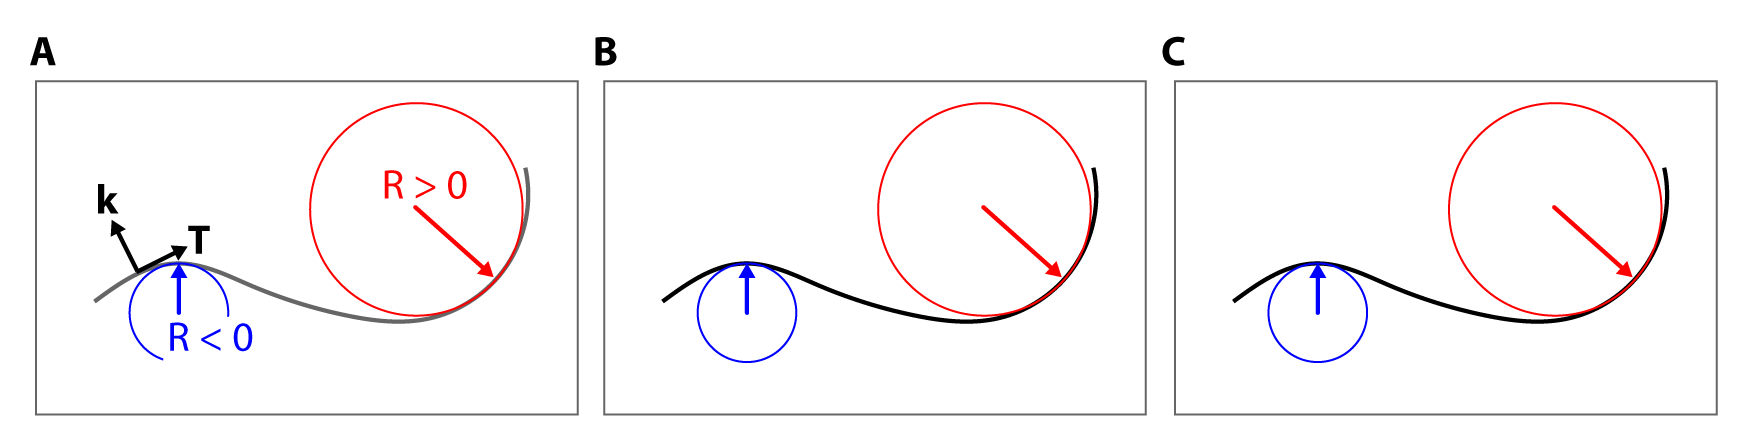
\includegraphics{figures/C1/Ch1-Figs_Curvature.png}
  \caption{Planar and surface curvature.
  (A), A planar curve with unit tangent vector $\mathbf{T}$ and unit normal vector $\mathbf{k}$. The osculating circles and associated radii of curvature are given for two points on the curve; the negative curvature is in blue and the positive curvature in red.
  (B), A normal section of a saddle-surface surface at a point corresponds to a planar curve, with the curve drawn in dark gray and the plane indicated in transparent gray.
  The osculating circle and radius of curvature at the point of interest are drawn in blue.
  (C), The principal curvatures $\kappa_1$ and $\kappa_2$ at the point of interest on the surface from (B) are the maximum and minimum normal curvatures and are always in orthogonal directions. Here they are highlighted with the red and blue osculating circles and radii of curvature.}\label{f:1-Curvature}
\end{figure}

In addition, as demonstrated through our example of geometrical frustration, Gaussian curvature must also couple to the free energy of an orientationally ordered phase confined to a surface.
In fact, for a topological charge density
\begin{equation}
  \rho(\mathbf{r}) = 2 \pi \sum\limits_i s_{i}\delta(\mathbf{r} - \mathbf{r}_{i}),\label{e:1-ChargeDens}
\end{equation}
with disclinations indexed by $i$ possessing charge $s_{i}$ and position $\mathbf{r}_{i}$, and $\delta(\mathbf{r} - \mathbf{r}_{i})$ the Kronecker delta function, we can express Eq~\ref{e:2-XY} as~\cite{RN42,RN175,RN17}:
\begin{equation}
  F_d = -\frac{1}{2} k_f \int \textrm{d}^2\mathbf{r} \, \textrm{d}^2\mathbf{r}' \, G_L(\mathbf{r},\mathbf{r}') [\rho(\mathbf{r})-K(\mathbf{r})] [\rho(\mathbf{r}')-K(\mathbf{r}')],\label{e:1-TopTheoryofDefects}
\end{equation}
where $G_L$ is the Green's function of the Laplace-Beltrami operator, the standard Laplacian operator generalized to curved space~\cite{RN17}.
It is worth mentioning that Eq.~\ref{e:1-TopTheoryofDefects} is identical to the Coulomb energy of a multicomponent plasma with charge density $\rho$ in a background of charge density $-K$~\cite{RN17}.
Thus, from the continuum theory, we see topological defects emerge as particle-like objects that possess topological charge and couple to the Gaussian curvature of the underlying substrate.

Importantly, this implies that even though there have been new discoveries as a result of examining defect structures on spheres~\cite{RN106,RN26,RN110,RN76,RN101,RN165}, including our prior work with spherical nematic shells highlighted earlier~\cite{RN45,RN105}, the Gaussian curvature and therefore the background topological charge density of a sphere is constant such that the impact of curvature can only enter through the sphere radius.
This is borne out in both the size-dependent onset of grain-boundary scars in colloidal crystals on the surface of emulsion drops~\cite{RN26,RN110}, and in the fact that the positions of the four $s = +1/2$ defects in nematic shells are due entirely to the defect-defect interactions alone~\cite{RN45}.
If we want to investigate the role of curvature on ordered materials, we need to consider a space with varying Gaussian curvature and ideally, Gaussian curvature of different sign.

The simplest closed surface that satisfies these criteria is the torus [Figure~\ref{f:1-ChiObjects}(C)], with $g = 1$ and thus $\chi = 0$.
In addition, we see that not only does a torus have sphere-like positive Gaussian curvature on the outer portion of the handle and saddle-like negative Gaussian curvature on the inner portion of the handle, but according to Eq~\ref{e:1-GB2}, the integrated Gaussian curvature over an entire torus must vanish.
Similarly, by Eq.~\ref{e:1-PH}, an orientationally ordered material on the surface of a torus must have vanishing topological charge and thus can support a defect-free configuration.

Prior work in our group investigated nematic order on the surface of a torus using toroidal droplets made from a NLC, with the NLC constrained to lie parallel to the interface between the toroidal droplet and the outer continuous medium~\cite{RN24,RN47}.
Like the thick spherical shells or a bipolar droplet, here we have a 3D nematic that must minimize its free energy in the presence of a constraint on the topological charge on the 2D confining surface.
While we found that toroidal droplets have a defect-free ground state, the varying curvature still led to new insights about the role of a distortion called saddle-splay.
Specifically, we found that saddle-splay drives the director in the plane of the surface to align along the smallest principle curvature~\cite{RN59}, yielding a doubly-twisted ground state in our toroidal droplets~\cite{RN24}, as drawn for both a left-handed twist and a right-handed twist in Figure~\ref{f:1-Torus}(A,B), respectively.
We found that the amount of twist in the ground state can be controlled by the aspect ratio, or slenderness of the torus $\xi = R_0/a$, with $R_0$ the radius of the central circle of the torus and $a$ the tube radius of the torus, as defined in Figure~\ref{f:1-Torus}(C).
In addition, as seen by the possibility of having either a left-handed or right-handed twist [Figure~\ref{f:1-Torus}(A,B)], this doubly-twisted state manifests itself through a spontaneous reflection symmetry breaking, where the free energy resembles that of the Landau theory of magnetism.
In fact, in the cylindrical limit where $\xi \rightarrow \infty$, the free energy of our doubly-twisted director ansatz has exactly the functional form of the Landau theory of magnetism~\cite{RN293}.
This is an example of how confinement can affect a system, even in the absence of defects.
\begin{figure}
  \centering
  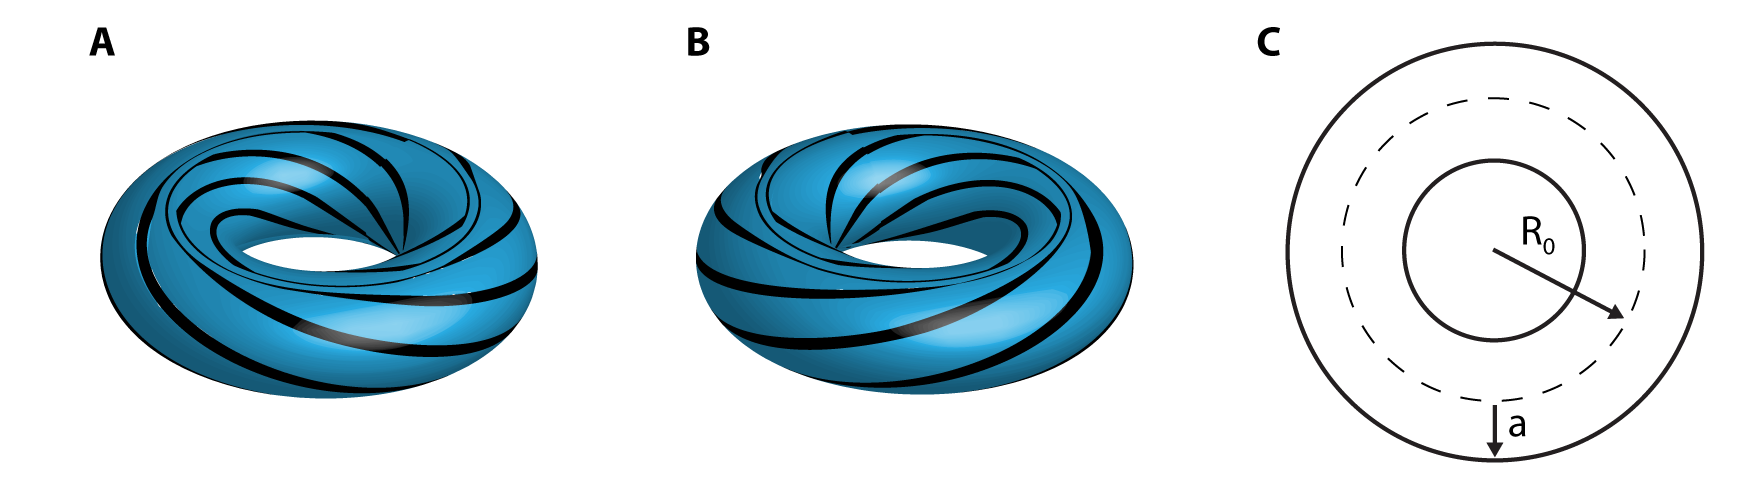
\includegraphics{figures/C1/Ch1-Figs_Torus.png}
  \caption{Doubly-twisted tori.
  (A,B), Schematics showing a (A) left-handed and (B) right-handed double-twist.
  (C), Schematic defining the central ring radius $R_0$ and tube radius $a$ in a torus.}\label{f:1-Torus}
\end{figure}

Up to this point we have considered how constraints imposed on order at a surface affect ordered materials that lie on the surface or are confined by the surface.
However, we can also use confinement to impose constraints on the bulk.
For example, consider the bipolar configuration where the director at the surface of a spherical droplet is forced to lie tangential to the surface.
If we instead require the director at the surface of the droplet to be perpendicular to the interface, known as homeotropic anchoring, we see that there must be an irreducible singularity in the bulk.
These bulk singularities are known as hedgehogs and are characterized by their hedgehog charge,
\begin{equation}
  q = \frac{1}{4 \pi} \int_{\mathbb{S}^2} d\theta \: d\phi \: \mathbf{n} \cdot \left [ \partial_{\theta} \mathbf{n} \times \partial_{\phi} \mathbf{n} \right ],\label{e:1-HedgehogCharge}
\end{equation}
where the integral is taken over a topologically spherical surface enclosing the defect, and $\theta$ and $\phi$ are, respectively, the polar and azimuthal angles on that surface~\cite{RN153}.
Instead of counting the number of times the director wraps around $\mathbb{S}^1$, as we do for the topological charge, here we consider the orientation of $\mathbf{n}$ on the spherical surface enclosing the defect mapped to $\mathbb{S}^2$, the unit sphere.
The hedgehog charge is then the number of times the orientations of $\mathbf{n}$ cover $\mathbb{S}^2$~\cite{RN153}.
Thus, we see that confining a NLC to a volume that is topologically spherical with homeotropic boundary conditions must yield a total ``hedgehog charge'' $|d|=1$.

In this Thesis, we investigate the role of geometry on the interplay between order and confinement.
In Chapter 2, we begin with an introduction to the theory of nematic liquid crystals.
Then, in Chapter 3, we consider nematic order on the surface of a torus.
Due to the difficulty of creating a thin, stable, toroidal shell of a NLC, we use a polymeric nematic that self-assembles at the interface between two immiscible liquids.
Importantly, this lets us make stable toroidal droplets as in our previous work, yet still investigate 2D nematic order on a toroidal surface.
In addition, the nematic is active, meaning that the individual constituent particles have their own source of internal energy.
The activity then drives the nematic out of equilibrium at the individual particle level, generally filling the nematic with pairs of $s = \pm 1/2$ defects that are constantly in motion and constantly being created and annihilated.
Even though we have an inherently nonequilibrium material, we find that predictions built upon Eq.~\ref{e:1-TopTheoryofDefects} hold and that adding activity to order qualitatively resembles bringing an equilibrium system to the high temperature limit.

In Chapter 4, we consider NLC confined to toroidal droplets under homeotropic boundary conditions.
With the director constrained to lie perpendicular to the surface, the saddle-splay distortion does not affect the free energy minimization.
However, we still find a twisted ground-state configuration, where the amount of twist depends on $\xi$, eventually disappearing as $\xi \rightarrow \infty$.
Experiments with NLC confined to straight and bent cylindrical capillaries under homeotropic boundary conditions reveal that the twist is a response to the additional curvature induced when deforming a cylinder of homeotropic nematic into a torus.
In Chapter 5, we return to a spherical topology, confining NLC to a capillary bridge with homeotropic anchoring to study the influence of confinement shape on defect type.
% Finally, in Chapter 6, we use toroids and spherical droplets to uncover the role of surface curvature of the anchoring of NLC.
In Chapter 6, we summarize our results and indicate potential future work that builds on this Thesis.
